%%%% Better Poster latex template example v1.0 (2019/04/04)
%%%% GNU General Public License v3.0
%%%% Rafael Bailo
%%%% https://github.com/rafaelbailo/betterposter-latex-template
%%%% 
%%%% Original design from Mike Morrison
%%%% https://twitter.com/mikemorrison

\documentclass[a0paper,fleqn]{betterposter}

%%%% Keep the original BetterPoster layout.
\setlength{\leftbarwidth}{0.3\paperwidth}
\setlength{\rightbarwidth}{0.3\paperwidth}

%%%% Poster-scale typography.
\renewcommand{\fontsizestandard}{\fontsize{27}{36} \selectfont}
\renewcommand{\fontsizemain}{\fontsize{76}{92} \selectfont}
\renewcommand{\fontsizetitle}{\fontsize{50}{60} \selectfont}
\renewcommand{\fontsizeauthor}{\fontsize{20}{26} \selectfont}
\renewcommand{\fontsizesection}{\fontsize{30}{38} \selectfont}

%%%% Blue central panel.
\renewcommand{\maincolumnbackgroundcolor}{imperialblue}

\graphicspath{{../paper/figures/}}

\newcommand{\MCBE}{M-CBE}
\newcommand{\LinMCBE}{Lin-M-CBE}
\newcommand{\SymMCBE}{Sym-M-CBE}
\newcommand{\sidebody}[1]{{\fontsize{22}{29}\selectfont #1}}
\newcommand{\tinycap}[1]{{\fontsize{15}{18}\selectfont\color{gray}#1}}
\newcommand{\fullfig}[3]{%
\begin{center}
\includegraphics[width=#1\linewidth]{#2}

\tinycap{#3}
\end{center}
}

\begin{document}
\betterposter{
%%%%%%%% MAIN COLUMN
\maincolumn{
\begin{center}
{\fontsize{68}{82}\selectfont
\textbf{Explain what the model sees}\\
\textbf{and how it reasons.}}

\vspace{0.65cm}
{\fontsize{34}{43}\selectfont
Human concepts + readable mechanisms,\\
at the complexity users choose.}

\vspace{0.9cm}
\begin{tikzpicture}
    \node[inner sep=0pt] (method) at (0,0) {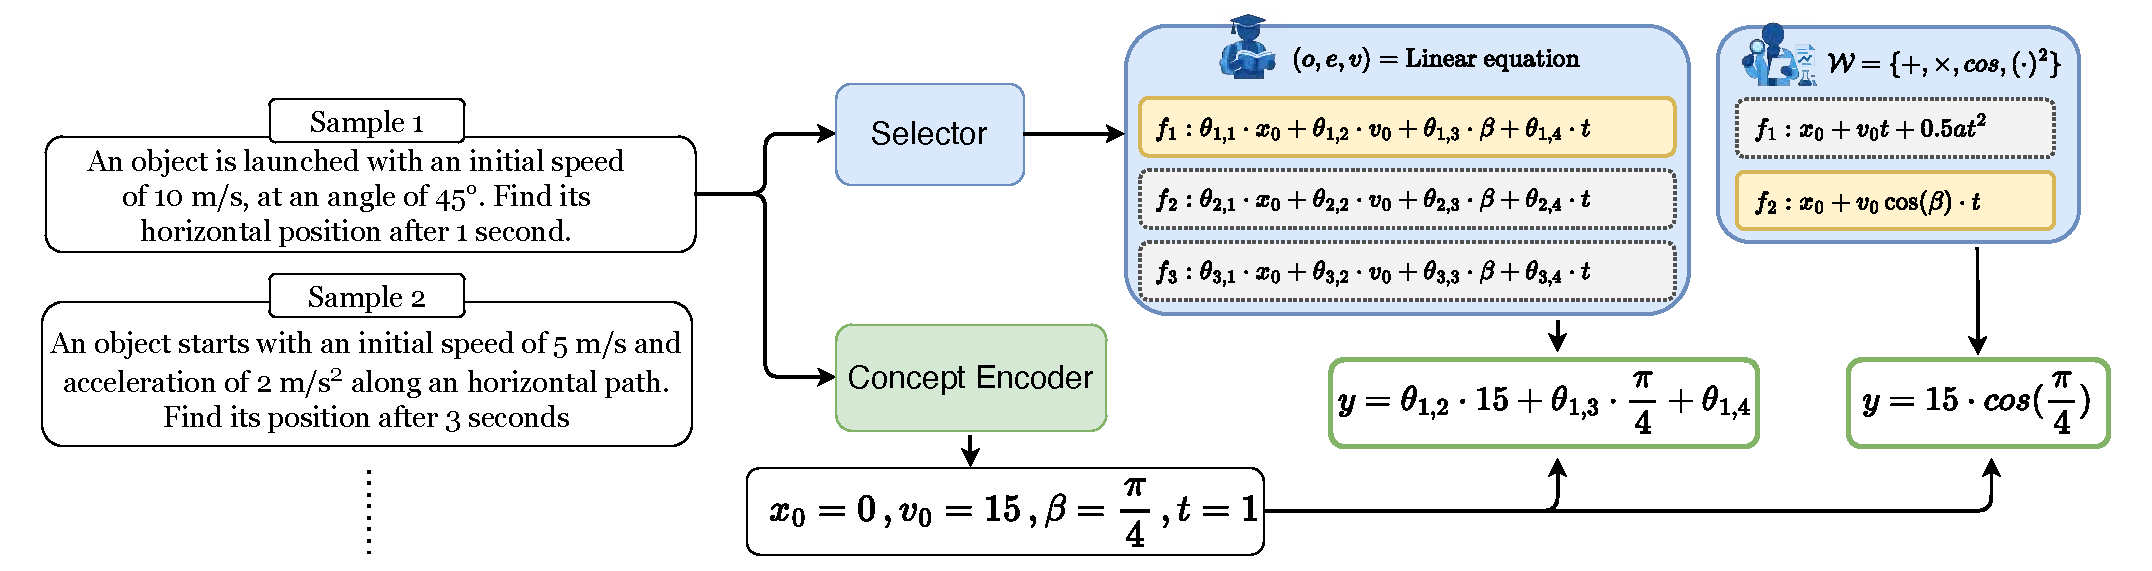
\includegraphics[width=0.98\linewidth]{method-compressed.pdf}};

    \node[fill=white, text=imperialblue, text width=6.2cm, align=center, inner sep=0.28cm] (what) at (-7.2,2.25) {\fontsize{19}{23}\selectfont\textbf{WHAT}\\ human-readable concepts};
    \node[fill=white, text=imperialblue, text width=6.4cm, align=center, inner sep=0.28cm] (how) at (0,2.25) {\fontsize{19}{23}\selectfont\textbf{HOW}\\ selected mechanism};
    \node[fill=white, text=imperialblue, text width=6.7cm, align=center, inner sep=0.28cm] (knob) at (7.3,2.25) {\fontsize{19}{23}\selectfont\textbf{USER KNOB}\\ linear or symbolic, simple or rich};

    \node[circle, fill=imperialblue, text=white, inner sep=0.18cm] at (-5.1,0.55) {\fontsize{18}{20}\selectfont\textbf{1}};
    \node[circle, fill=imperialblue, text=white, inner sep=0.18cm] at (-0.55,0.40) {\fontsize{18}{20}\selectfont\textbf{2}};
    \node[circle, fill=imperialblue, text=white, inner sep=0.18cm] at (5.5,0.40) {\fontsize{18}{20}\selectfont\textbf{3}};
\end{tikzpicture}
\end{center}
}{
\begin{center}
{\fontsize{27}{35}\selectfont
\textbf{Mixture of Concept Bottleneck Experts} exposes both the variables and the mechanisms behind a prediction.}

\vspace{0.65cm}
\qrset{link, height=0.14\linewidth}
\tikz \node[rectangle, draw, inner sep=.30cm, fill=white] {\color{black}\qrcode{https://github.com/francescoTheSantis/Mixture-of-CB-Experts}};

{\fontsize{19}{24}\selectfont Code and experiments}
\end{center}
}
}{
%%%%%%%% LEFT COLUMN
\title{Mixture of Concept Bottleneck Experts}

{\fontsize{20}{26}\selectfont\color{gray}
Francesco De Santis, Gabriele Ciravegna, Giovanni De Felice, Arianna Casanova, Francesco Giannini, Michelangelo Diligenti, Johannes Schneider, Danilo Giordano, Mateo Espinosa Zarlenga, Pietro Barbiero
}

\vspace{0.35cm}
\institution{ICML 2026}

\section{Why}
\sidebody{Concept-based models can tell us \textbf{which human variables} matter, but often hide or over-fix \textbf{the mechanism} that turns those variables into a prediction.}

\section{Core Idea}
\sidebody{\MCBE{} learns a \textbf{finite menu of readable mechanisms}. Each prediction selects one mechanism, and each mechanism uses only predicted concepts.}

\section{Two Axes of Control}
\begin{center}
\begin{minipage}{0.48\linewidth}
\centering
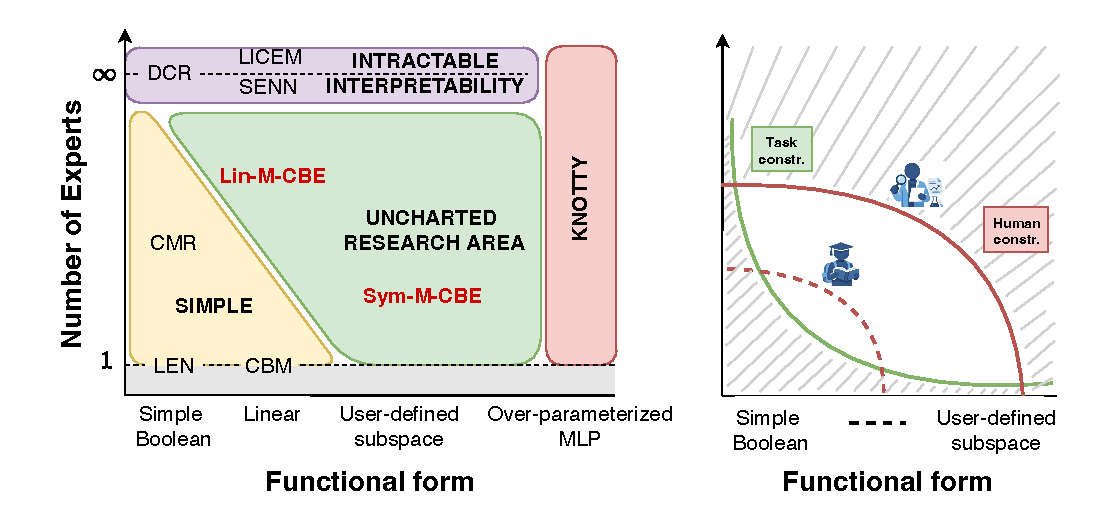
\includegraphics[width=\linewidth,trim=0cm 0cm 9.45cm 0cm,clip]{visual_abstract.pdf}

\tinycap{Choose the functional language.}
\end{minipage}
\hfill
\begin{minipage}{0.48\linewidth}
\centering
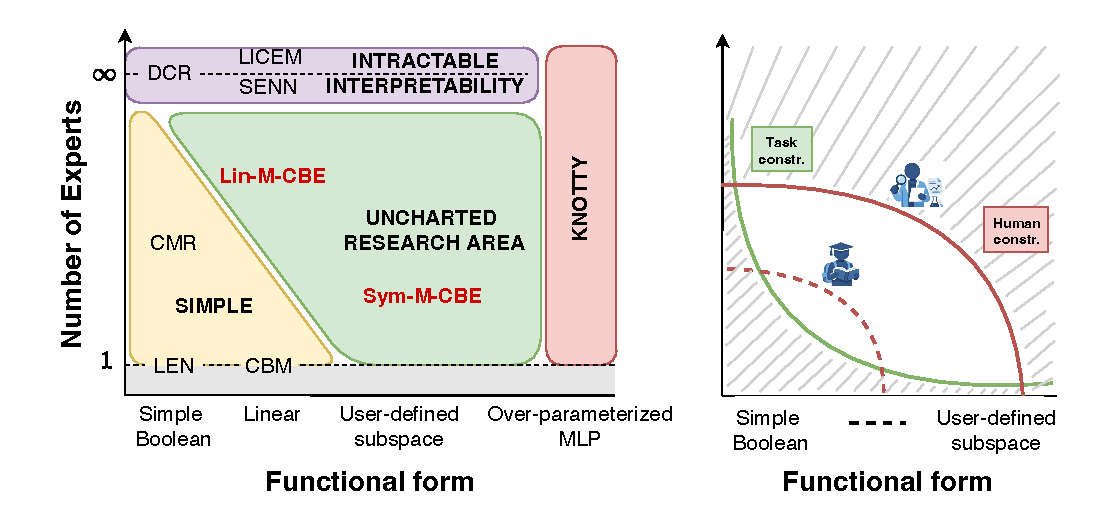
\includegraphics[width=\linewidth,trim=9.45cm 0cm 0cm 0cm,clip]{visual_abstract.pdf}

\tinycap{Choose the feasible complexity.}
\end{minipage}
\end{center}

\section{Interpretability}
\begin{center}
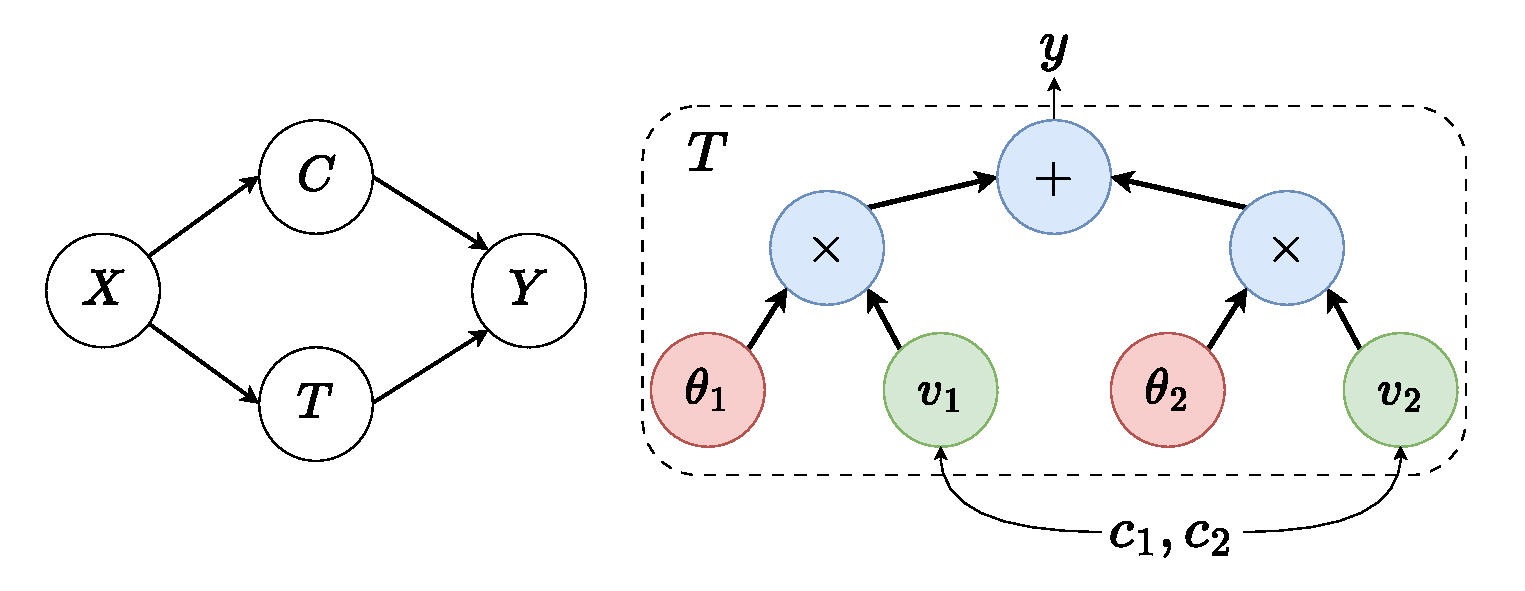
\includegraphics[width=0.49\linewidth]{pgm_exp_tree.pdf}
\hfill
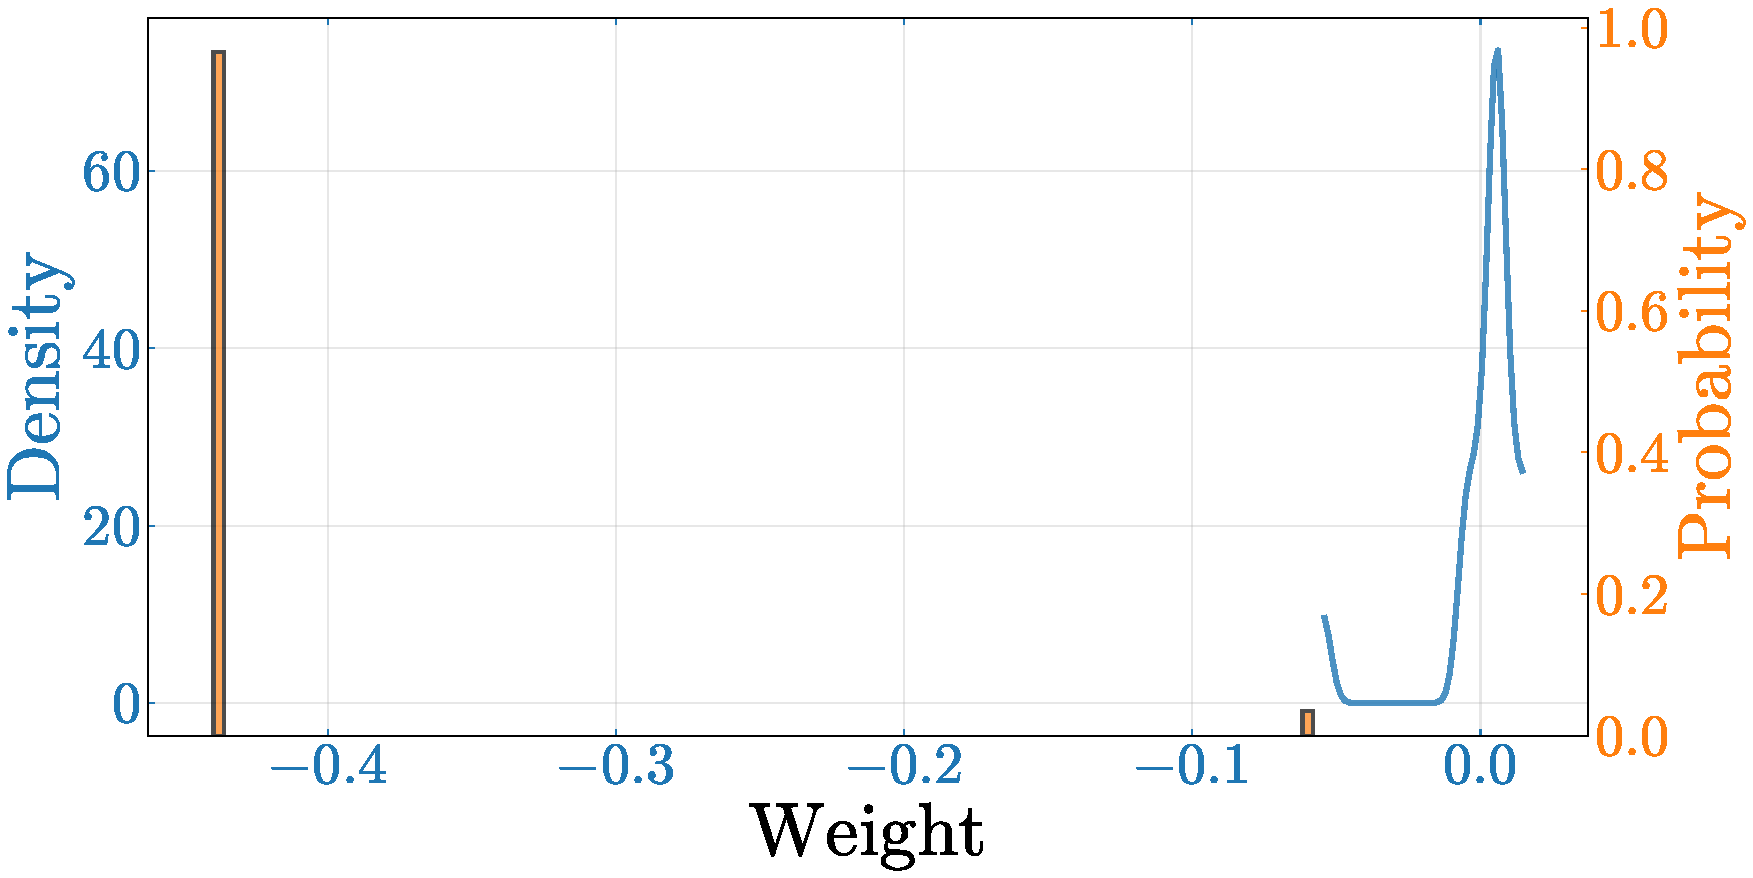
\includegraphics[width=0.49\linewidth]{global_verifiability.pdf}

\tinycap{Expression trees make mechanisms inspectable; finite experts make global verification possible.}
\end{center}

\section{Instances}
\sidebody{\textbf{\LinMCBE}: multiple linear mechanisms.\\
\textbf{\SymMCBE}: symbolic mechanisms under user-chosen operators.}
}{
%%%%%%%% RIGHT COLUMN
\section{Experiments}
\sidebody{Nine benchmarks: regression and classification, continuous and discrete concepts, complete and incomplete bottlenecks, plus label-free concepts.}

\fullfig{0.94}{pareto_front.pdf}{Accuracy vs. complexity. Changing both mechanism language and number of experts reveals better trade-offs.}

\fullfig{0.94}{pareto_int.pdf}{Concept interventions. Mechanism-aligned experts recover performance when users correct concepts.}

\fullfig{0.88}{concept_size_ablation.pdf}{Scalability. Flexible algebraic mechanisms remain robust as concept sets grow.}

\fullfig{0.92}{interventions_ood.pdf}{OOD interventions. Finite mechanisms limit leakage and stay responsive under noisy inputs.}

\begin{center}
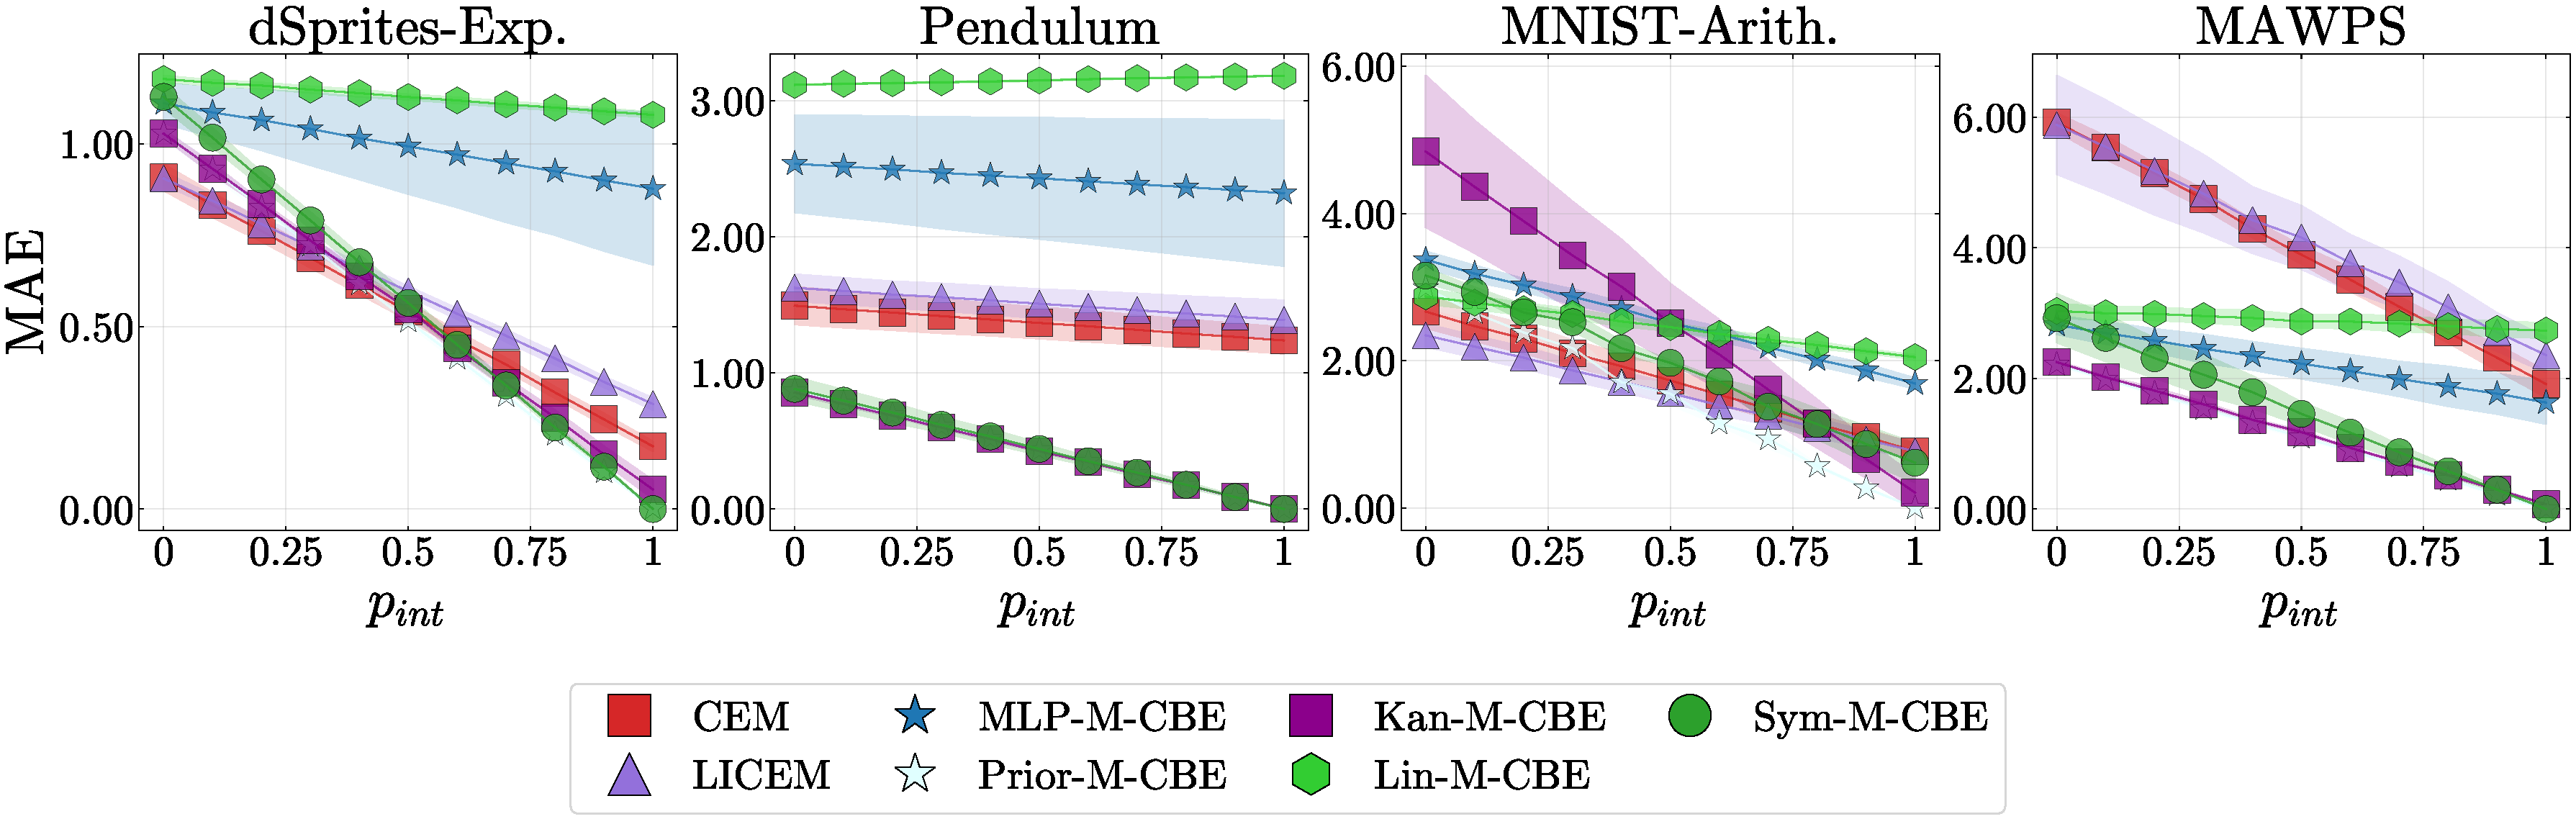
\includegraphics[width=0.48\linewidth]{sr_ablation_int.pdf}
\hfill
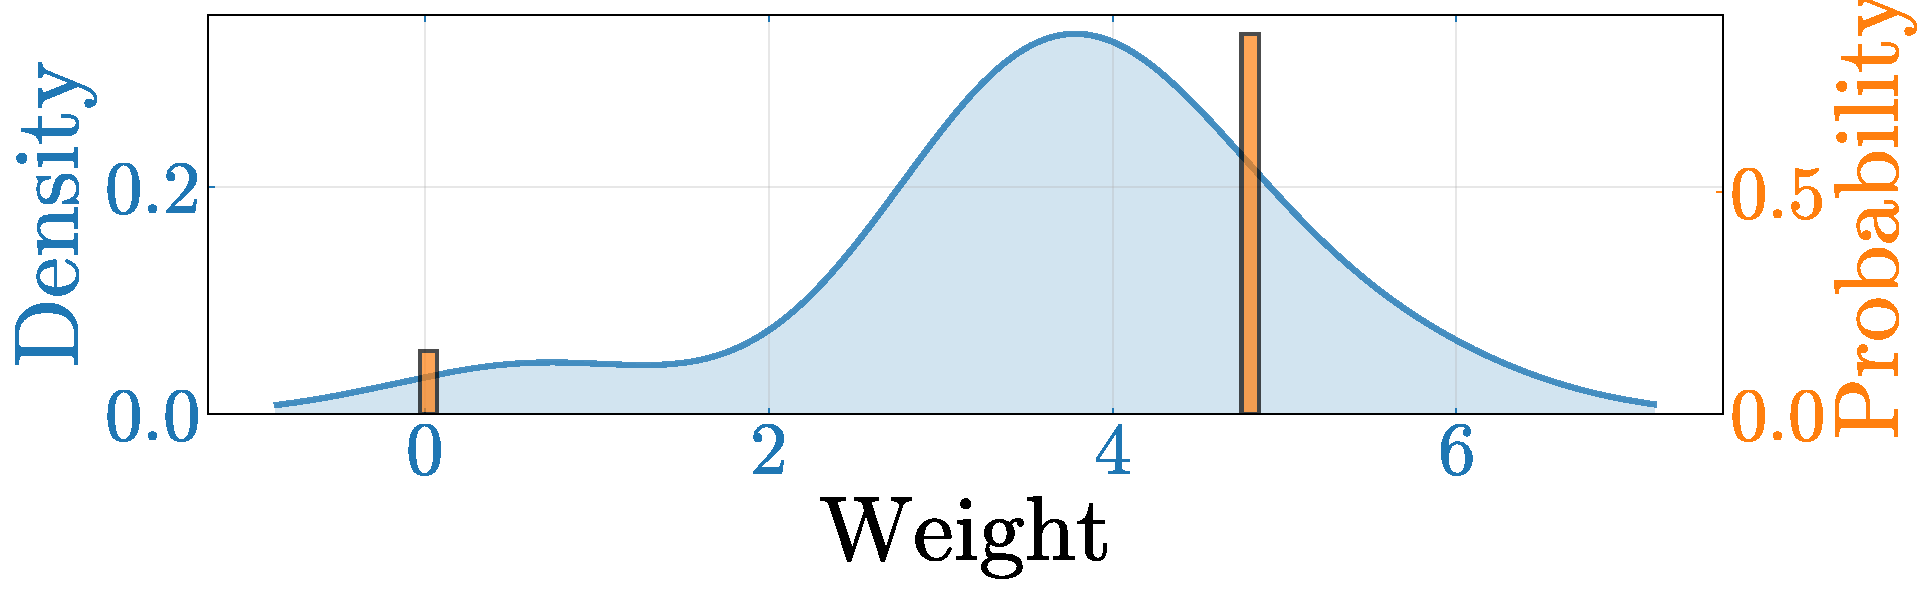
\includegraphics[width=0.48\linewidth]{has_underparts_color_brown_Crested_Auklet.pdf}

\tinycap{Symbolic ablation and an example of discrete, inspectable expert weights.}
\end{center}
}
\end{document}
